%% LyX 2.3.6 created this file.  For more info, see http://www.lyx.org/.
%% Do not edit unless you really know what you are doing.
\documentclass[english,aspectratio=169]{beamer}
\usepackage{lmodern}
\renewcommand{\sfdefault}{lmss}
\renewcommand{\ttdefault}{lmtt}
\usepackage[T1]{fontenc}
\usepackage[latin9]{inputenc}
\setlength{\parskip}{\medskipamount}
\setlength{\parindent}{0pt}
\usepackage{babel}
\usepackage{amstext}
\usepackage{amssymb}
\usepackage{graphicx}
\PassOptionsToPackage{normalem}{ulem}
\usepackage{ulem}
\ifx\hypersetup\undefined
  \AtBeginDocument{%
    \hypersetup{unicode=true}
  }
\else
  \hypersetup{unicode=true}
\fi

\makeatletter

%%%%%%%%%%%%%%%%%%%%%%%%%%%%%% LyX specific LaTeX commands.
\pdfpageheight\paperheight
\pdfpagewidth\paperwidth


%%%%%%%%%%%%%%%%%%%%%%%%%%%%%% Textclass specific LaTeX commands.
% this default might be overridden by plain title style
\newcommand\makebeamertitle{\frame{\maketitle}}%
% (ERT) argument for the TOC
\AtBeginDocument{%
  \let\origtableofcontents=\tableofcontents
  \def\tableofcontents{\@ifnextchar[{\origtableofcontents}{\gobbletableofcontents}}
  \def\gobbletableofcontents#1{\origtableofcontents}
}

%%%%%%%%%%%%%%%%%%%%%%%%%%%%%% User specified LaTeX commands.
%\usetheme{CambridgeUS}
%\usetheme{Singapore}
\usetheme{Warsaw}
\usecolortheme{beaver}
\hypersetup{pdfpagemode=None}
\usepackage{tikz}
\usepackage{color}
\usepackage{listings}
\usepackage{multicol}
\setbeamertemplate{footline}[frame number]

\makeatother

\begin{document}
\title[Intro BGCM]{Introduction to (biogeochemical) modelling}
\author{Prof. Marcello Vichi}
\institute[UCT]{Department of Oceanography\\University of Cape Town\\marcello.vichi@uct.ac.za}
\date{SEA2005S}
\makebeamertitle

\section*{Outline}
\begin{frame}{Outline of the Course}

\begin{multicols}{2}\tableofcontents{}\end{multicols}
\end{frame}


\section{Introduction to modelling in marine systems}

\subsection{What is a model}

\frame{\subsectionpage}
\begin{frame}{Mathematical modelling}

\begin{itemize}
\item \textbf{\footnotesize{}Mathematical modelling}{\footnotesize{} is
the process of defining }{\footnotesize{}\uline{system state variables}}{\footnotesize{}
and }{\footnotesize{}\uline{drivers}}{\footnotesize{} ,by constructing
appropriate functional relationships between them (i.e. how variables
respond to drivers) }{\footnotesize\par}
\item {\footnotesize{}This activity includes the various methods to understand
conceptual relationships, write mathematical }\textbf{\footnotesize{}parameterizations}{\footnotesize{}
(or physical laws if known), and eventually use the equations in simulations
and predictions}{\footnotesize\par}
\item {\footnotesize{}Applications of a model require that the modeller
knows enough about the process to construct expressions about the
real-world variables (Lassiter, 1975)}{\footnotesize\par}
\end{itemize}
\begin{definition}[]
{\footnotesize{}A }\textbf{\footnotesize{}process model}{\footnotesize{}
is a relationship between variables usually derived through empirical
methods (a statistical model).}{\footnotesize\par}

{\footnotesize{}A }\textbf{\footnotesize{}dynamical model}{\footnotesize{}
is a set of differential equations based on process models that describe
the evolution of a system in time and space.}{\footnotesize\par}
\end{definition}

\end{frame}

\begin{frame}{Parameter: the multi-purpose word}

\begin{definition}
{\footnotesize{}A }\emph{\footnotesize{}parameter}{\footnotesize{}
is an argument of a function that is considered constant}{\footnotesize\par}
\end{definition}

\begin{itemize}
\item {\footnotesize{}However, parameter is a multi-purpose word that can
be used in different contexts. Functions have several arguments: the
ones that change (variables) and the ones that are constant (the parameters).
Sometimes a parameter may become a variable and vice versa, depending
on the assumptions}{\footnotesize\par}
\item \textbf{\footnotesize{}Parameterization}{\footnotesize{} is a buzzword
in earrth sciences. A process is parameterized when a mathematical
function (a curve and its constant parameters) is specified by means
of one variable that is considered independent, and it is known to
drive a response on the variable of interest. It can be a function
of more variables. }\emph{\footnotesize{}A parameterization is an
approximated model of how a variable responds to inputs, without necessarily
including all the mechanistic details}{\footnotesize{}.}{\footnotesize\par}
\item {\footnotesize{}Finally, in oceanography and atmospheric sciences
the variables are often called parameters when they are measured instrumentally
(e.g. the measured parameters were 10 m wind velocity, specific humidity,
sea surface temperature and salinity).}{\footnotesize\par}
\end{itemize}
\end{frame}

\begin{frame}{State variables, drivers and processes: which is which?}

\begin{itemize}
\item Nutrient uptake in phytoplankton is a function of concentration in
the surrounding water
\item Primary production in the ocean is a function of vertical mixing (light
availability), temperature, and nutrient availability
\item Zooplankton predation is a function of available preys and search
efficiency
\item Others?
\end{itemize}
\begin{alertblock}{Do they sound true but vague?}
A quantitative approach is necessary to define and express these
relationships
\end{alertblock}
\end{frame}

\begin{frame}{Environmental drivers}

\textbf{A driver is a state variable}. It is used to \uline{drive}
component(s) of a system (i.e. other state variables) as an external
condition, also known as one-way forcing. 

Environmental (or abiotic) drivers are identifiable physical features
of the marine system, such as salinity, temperature, mixing, others?
In the real marine system, there can be two-way forcings, feedback
between state variables that affect the drivers (phytoplankton absorb
light and changes the temperature of the ocean). \textbf{Environmental
drivers} come from:
\begin{itemize}
\item In situ observations (SEA2004F)
\item Earth observations (SEA2004F)
\item Model generated (ocean or climate numerical models)
\end{itemize}
\begin{alertblock}{What is an ocean model?}
Let's ask AI...
\end{alertblock}
\end{frame}
%
\begin{frame}{A quick view at ocean and climate models}
\begin{columns}[t]


\column{6cm}
\begin{itemize}
\item {\small{}What is a climate model? }{\small{}\uline{\href{https://www.carbonbrief.org/qa-how-do-climate-models-work/}{Carbonbrief.org}}}{\small{} }{\small\par}
\item {\small{}Ocean numerical models }{\small{}\uline{\href{https://noc.ac.uk/education/educational-resources/ocean-science-action/introduction-ocean-modelling-its-all-numbers\#top}{noc.ac.uk}}}{\small\par}
\item {\small{}Blue, green, and white ocean models }{\small{}\uline{\href{https://marine.copernicus.eu/explainers/operational-oceanography/monitoring-forecasting/models}{marine.copernicus.eu}}}{\small\par}
\item {\small{}Ocean products visualization }{\small{}\uline{\href{https://marine.copernicus.eu/access-data/ocean-visualisation-tools}{marine.copernicus.eu}}}{\small\par}
\end{itemize}

\column{6cm}

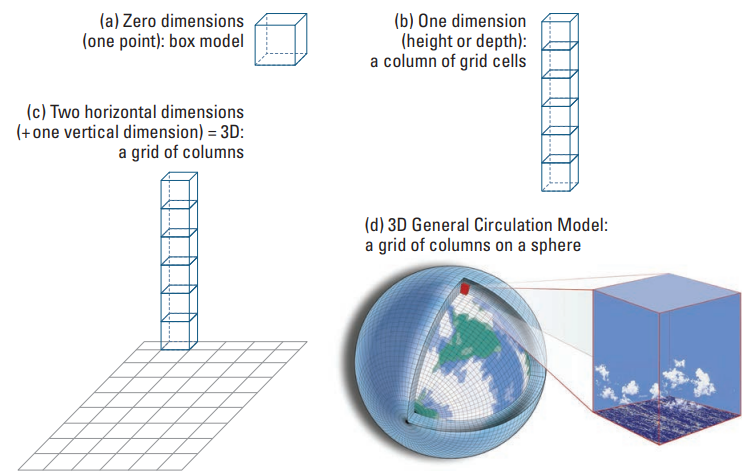
\includegraphics[scale=0.45]{figures/0-3D_grids}
\end{columns}

\end{frame}
%

\subsection{Green ocean models}

\frame{\subsectionpage}

\begin{frame}{The green ocean: a quantitative description for biogeochemistry}
\begin{itemize}
\item In marine chemical-biological systems, problems are often more complex
than in purely physical systems. The governing equations of the chemical-biological
dynamics cannot be derived explicitly from conservation laws as in
Newton's mechanics or in geophysical fluid dynamics. 
\item These equations must be derived from observations. Experimental findings
can be translated into mathematical formulations, which describe the
process quantitatively. These functions represent the \textbf{response
curves (or reaction norms)} and the interactions between drivers and
state variables. The combination of these formulations constitutes
a dynamical model.
\end{itemize}
\end{frame}

\begin{frame}{A model of primary production in the ocean}

{\footnotesize{}This is the output of a numerical ocean-biogeochemistry
model applied to simulate the observed}\textbf{\footnotesize{} integrated
primary production}{\footnotesize{} at the Bermuda Atlantic Time Series
(BATS). The comparison is done using monthly means (}{\footnotesize{}\uline{\href{https://bg.copernicus.org/articles/6/2333/2009/}{Vichi and Masina, 2009}}}{\footnotesize{}).
This output is the result of multiple interactive process models that
generate an emergent behavior: the seasonal cycle of PP. }\textbf{\scriptsize{}Q:
What is integrated primary production? What are the drivers? At which
temporal and spatial scales are they expected to change?}{\scriptsize\par}

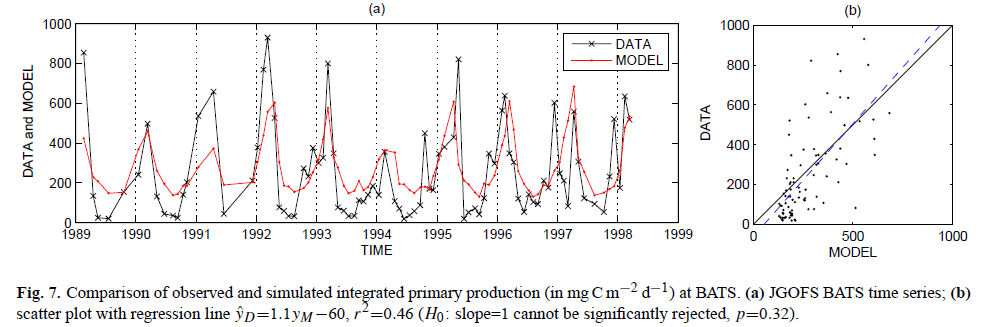
\includegraphics[width=0.9\paperwidth]{figures/PP_BATS} 
\end{frame}

\begin{frame}{Response curves (reaction norms)}

\begin{columns}[t]


\column{6cm}
\begin{itemize}
\item {\footnotesize{}A }\textbf{\footnotesize{}response curve}{\footnotesize{}
describes how certain species ``respond'' to one driver in laboratory
settings }{\footnotesize\par}
\item {\footnotesize{}The physiological response can be expressed in terms
of several indicator variables: photosynthetic rate, amount of oxygen
consumed, specific growth rate, nutrient uptake, etc. }{\footnotesize\par}
\item {\footnotesize{}For instance, in the Southern Ocean, temperature is
recognized to control the maximum growth rate of of diatoms. Other
drivers may also affect the realized growth, such as nutrients and
light. }{\footnotesize\par}
\end{itemize}

\column{6cm}

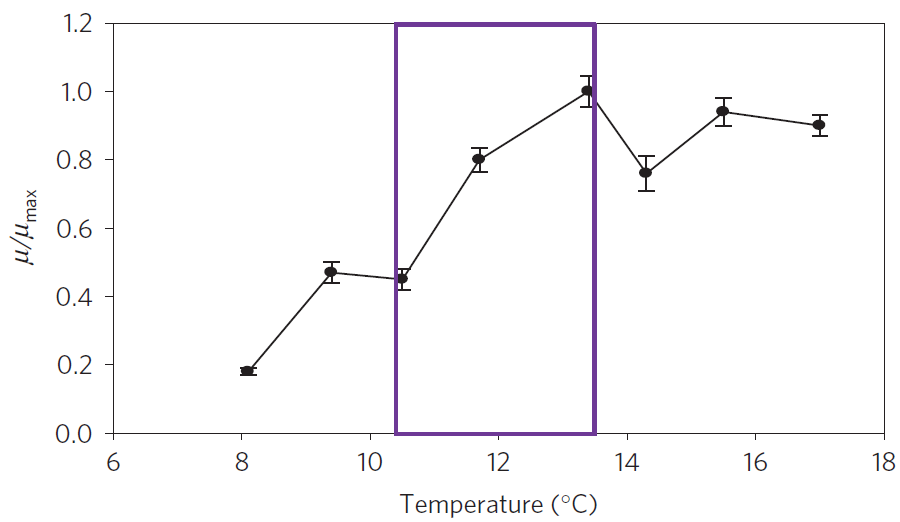
\includegraphics[scale=0.35]{figures/reaction_norm_T_boyd}

{\scriptsize{}A response curve of }\emph{\scriptsize{}Prorocentrum
multiseries}{\scriptsize{} (}{\scriptsize{}\uline{\href{https://www.nature.com/articles/nclimate2811}{Boyd et al., 2016}}}{\scriptsize{}).
Temperature bounds of the purple rectangle denote the mean (10.6$^{o}$C)
for sub-Antarctic surface waters for present-day spring/summer and
that projected (13.7$^{o}$C) for this province by 2100. }\textbf{\scriptsize{}Q:
do we expect surface waters in the Southern Ocean to be constantly
at this projected value?}{\scriptsize\par}
\end{columns}

\end{frame}

\begin{frame}{Macroscopic response to temperature}

\begin{columns}[t]

\column{6cm}

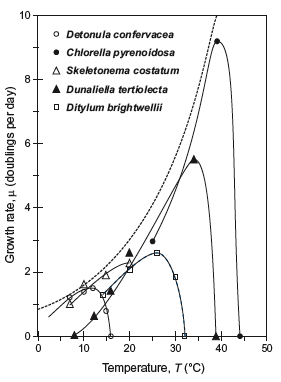
\includegraphics[width=5cm]{figures/eppley}

\column{7cm}
\begin{itemize}
\item {\footnotesize{}Physiological rates are controlled by environmental
temperature. }{\footnotesize\par}
\item {\footnotesize{}Eppley (}{\footnotesize{}\uline{\href{https://spo.nmfs.noaa.gov/sites/default/files/pdf-content/1972/704/eppley.pdf}{1972}}}{\footnotesize{})
demonstrated that single species are subject to temperature ranges
but taken as a population of algae in the ocean they are constrained
by a curve envelope. He proposed the empirical equation 
\[
\mu_{max}=0.59e^{0.0633T}
\]
}{\footnotesize\par}
\item {\footnotesize{}The Eppley equation gives the maximum potential growth
rate of the phytoplankton assemblage at each temperature. It is expressed
in doubling per day (related to the number of cells). }\textbf{\scriptsize{}Q:
Is this a response curve?}{\scriptsize\par}
\end{itemize}
\end{columns}

\end{frame}

\begin{frame}{Functional response to light}

\begin{columns}[t]

\column{9cm}
\begin{center}
\vspace{-0.7cm}
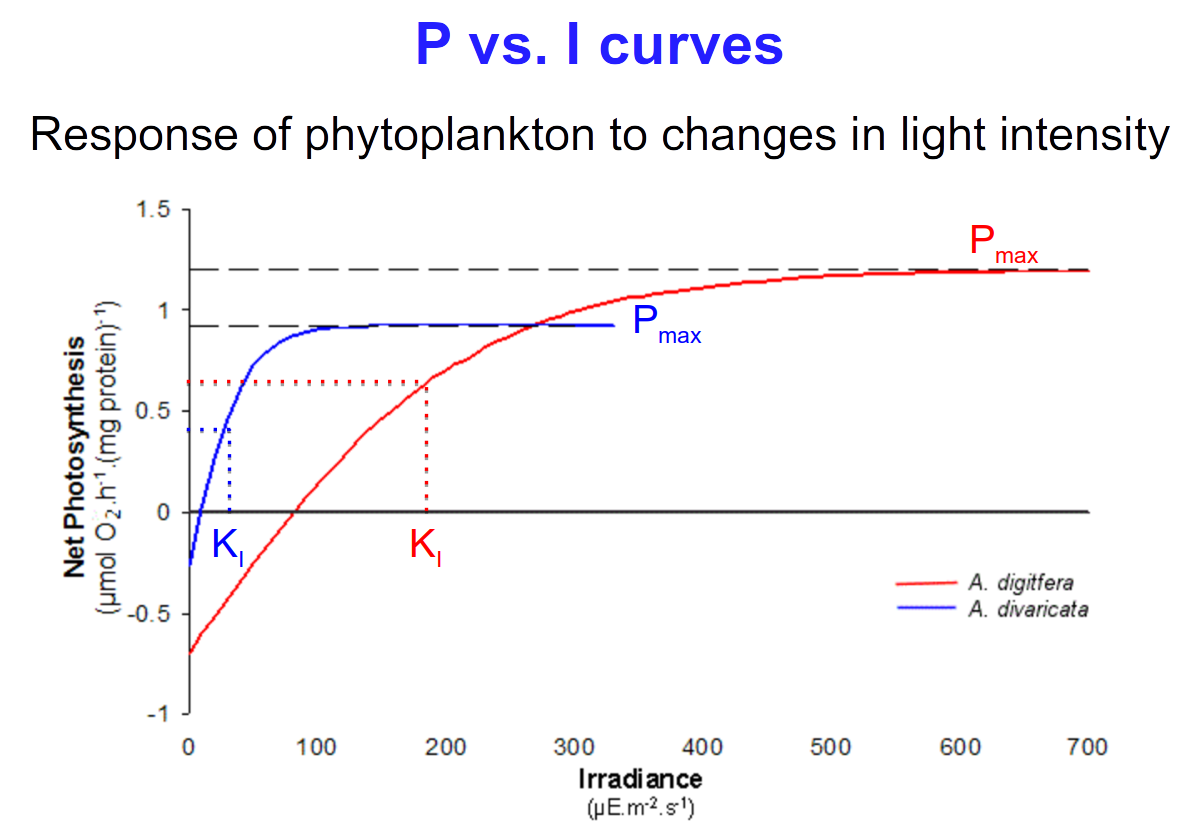
\includegraphics[width=5cm]{figures/P-I_Fawcett}\vspace{-0.7cm}
\par\end{center}
\begin{itemize}
\item {\scriptsize{}Several reaction norms have been proposed for phytoplankton
response to light (}{\scriptsize{}\uline{\href{https://aslopubs.onlinelibrary.wiley.com/doi/10.4319/lo.1976.21.4.0540}{Jassby and Platt, 1976}}}{\scriptsize{})}{\scriptsize\par}
\item {\scriptsize{}The hyperbolic shape you have seen in the earlier lectures
follows eq (2) 
\[
P\left(I\right)=P_{max}\alpha\frac{I}{\alpha I+P_{max}}
\]
 where $\alpha$ is the linear slope of the curve in under-saturated
light conditions and $I$ is the irradiance. }\textbf{\emph{\scriptsize{}Q:
Where is the half-saturation constant $K$in this equation?}}\textbf{\scriptsize{}
What are the units of $\alpha$?}{\scriptsize\par}
\end{itemize}

\column{7cm}

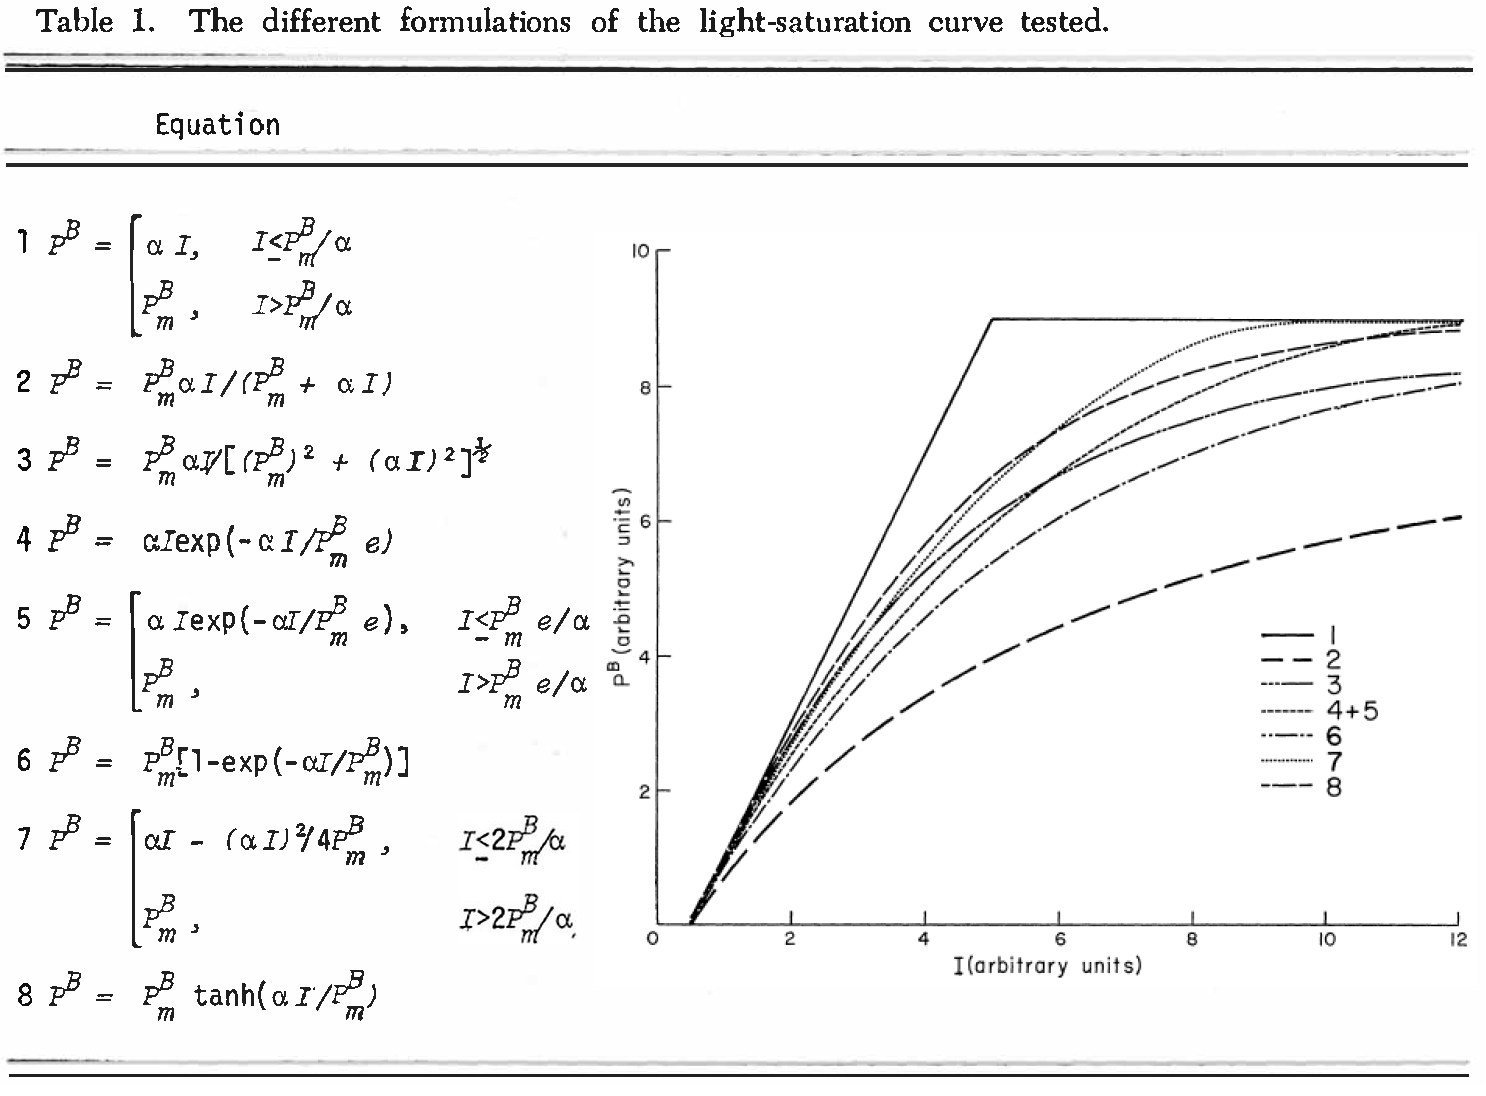
\includegraphics[width=7cm]{figures/jassby_platt}
\end{columns}

\end{frame}

\begin{frame}{Functional response to nutrients}

\begin{columns}[t]

\column{7cm}

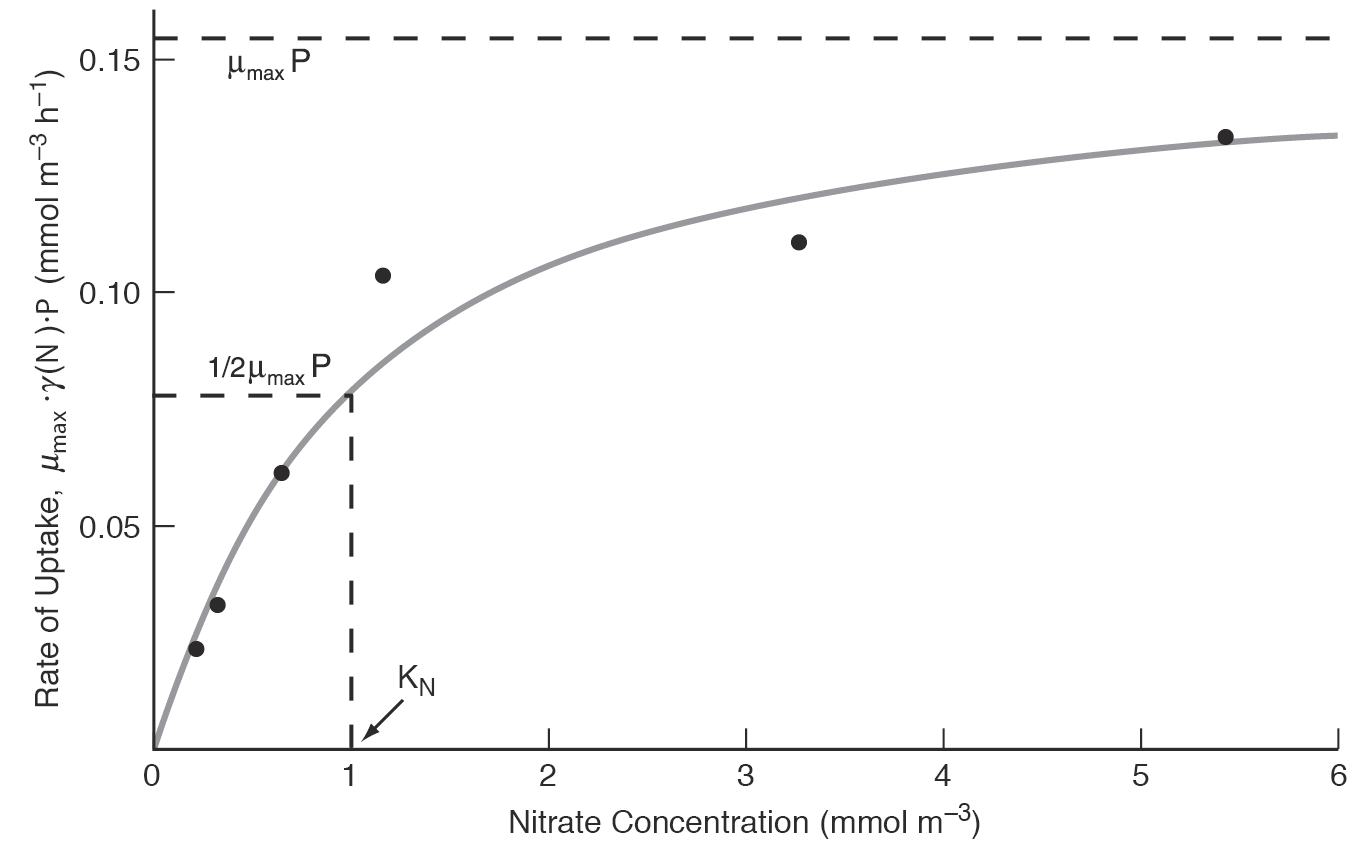
\includegraphics[width=7cm]{figures/MM}

\column{7cm}
\begin{itemize}
\item The \textbf{rate of uptake} of dissolved nutrients from the water
is a non-linear function of the environmental concentration. It's
a function on one single variable $N$, the concentration of the nutrient
(e.g. nitrate in mmol N m$^{-3}$)
\item Its functional form was proposed by \uline{\href{https://pubs.acs.org/doi/10.1021/bi201284u}{Michaelis and Menten (1913)}}
and \uline{\href{https://www.annualreviews.org/doi/10.1146/annurev.mi.03.100149.002103}{Monod (1949)}
}\textbf{\scriptsize{}Q: What are the units of the parameters? Which
part is unitless (non-dimensional)?}
\[
\mu\left(N\right)=\mu_{max}\frac{N}{N+K_{N}}
\]
\end{itemize}
\end{columns}

\end{frame}

\begin{frame}{Parameterization of a response curve}

\begin{columns}[t]


\column{6.5cm}
\begin{itemize}
\item {\footnotesize{}Organic carbon in the ocean is remineralized through
respiration. Also phytoplankton respiration depends on temperature.
Lassiter (1975) proposed a }\textbf{\footnotesize{}non-linear function}{\footnotesize\par}
\item {\footnotesize{}This continuous mathematical function is asymmetrical
with domain $\left]-\infty,+\infty\right[$; the curve is defined
by 2 major parameters: the optimal and maximum temperatures}
\[
f(x)=\begin{cases}
R_{0}e^{A\left(x-T_{opt}\right)}\left(\frac{T_{max}-x}{T_{max}-T_{opt}}\right)^{A\left(T_{max}-T_{opt}\right)} & x<T_{max}\\
0 & x\geq T_{max}
\end{cases}
\]
\end{itemize}

\column{7cm}


\includegraphics[width=5.5cm]{figures/respiration}

\textbf{\scriptsize{}Q: How do we visualize this curve on a graph?}{\scriptsize\par}
\end{columns}

\end{frame}


\section{Using mathematical functions to describe change }


\subsection{Describing the rate of change}

\frame{\subsectionpage}
\begin{frame}{Derivatives}

\begin{itemize}
\item <1->A function transforms a set of numbers into another set: mathematically,
we say that it maps a \textbf{domain} into a \textbf{co-domain} 
\item <2->Our brain can see patterns but is not automatically wired to
recognize mathematical functions. A graph of a function is the only
way to see ``what it does''
\item <3->In a function it is necessary to quantify these features:

\begin{itemize}
\item <3->the domain (range of validity): what are the values of $x$ where
$y=f(x)$ actually exists and has a realistic meaning?
\item <3->a measure of how much $y$ changes when the independent variable
$x$ changes. \textbf{For this we use calculus: the derivative}
\end{itemize}
\end{itemize}
\end{frame}

\begin{frame}{Computing derivatives: the respiration curve}

\begin{columns}[t]


\column{7cm}
\begin{itemize}
\item Respiration approximately doubles between 10 and 20$^{\circ}C$
\item $\frac{\Delta R}{\Delta T}=\frac{R(T=20)-R(T=10)}{10}=\frac{25-13.53}{10}=$
\textrm{}\\
\textrm{1.15} mg O$_{2}$ h$^{-1}$ $^{\circ}C^{-1}$
\item Let's now compute the rate of change every 5$^{\circ}C$ over the
same interval
\end{itemize}

\column{7cm}


\includegraphics[scale=0.35]{figures/respiration}

\end{columns}

\end{frame}

\begin{frame}{The derivative as a limit}

\begin{columns}[t]


\column{8cm}
\begin{itemize}
\item {\small{}The value of the rate varies with the choice of the interval}{\small\par}
\item {\small{}As we reduce the range of temperature, the change in respiration
with temperature will become smaller and will approach the ``instantaneous''
rate of change at a given temperature}{\small\par}
\item {\small{}For instance, the respiration rate at 10$^{\circ}C$ 
\[
\frac{\Delta R}{\Delta T}(10)=\lim_{\Delta T\rightarrow0}\frac{R(10+\Delta T)-R(10)}{\Delta T}
\]
will approach the tangent line as $\Delta T$ becomes smaller. The
derivative is positive or negative depending on the slope of the curve}{\small\par}
\end{itemize}

\column{6cm}


\includegraphics[scale=0.35]{figures/respiration_tangents}
\end{columns}

\end{frame}

\begin{frame}{General Rules}

\begin{enumerate}
\item The derivative of a sum is the sum of the derivatives: \\
$\frac{d}{dx}\left[F(x)+G(x)\right]=\frac{d}{dx}F(x)+\frac{d}{dx}G(x)$
\item The derivative of a product \textbf{IS\ NOT} the product of derivatives
but the cross-product: \\
$\frac{d}{dx}\left[F(x)G(x)\right]=\frac{dF}{dx}G+\frac{dG}{dx}F$
\item The derivative of a function of a function is the cross-derivative:\\
$\frac{d}{dx}G\left(F(x)\right)=\frac{dG}{dF}\frac{dF}{dx}$
\item {\scriptsize{}\uline{\href{http://www.dummies.com/how-to/content/the-most-important-derivatives-and-antiderivatives.html}{http://www.dummies.com/how-to/content/the-most-important-derivatives-and-antiderivatives.html}}}{\scriptsize\par}
\end{enumerate}
\end{frame}

\begin{frame}{Studying nonlinear functions}

\begin{columns}[t]

\column{6cm}

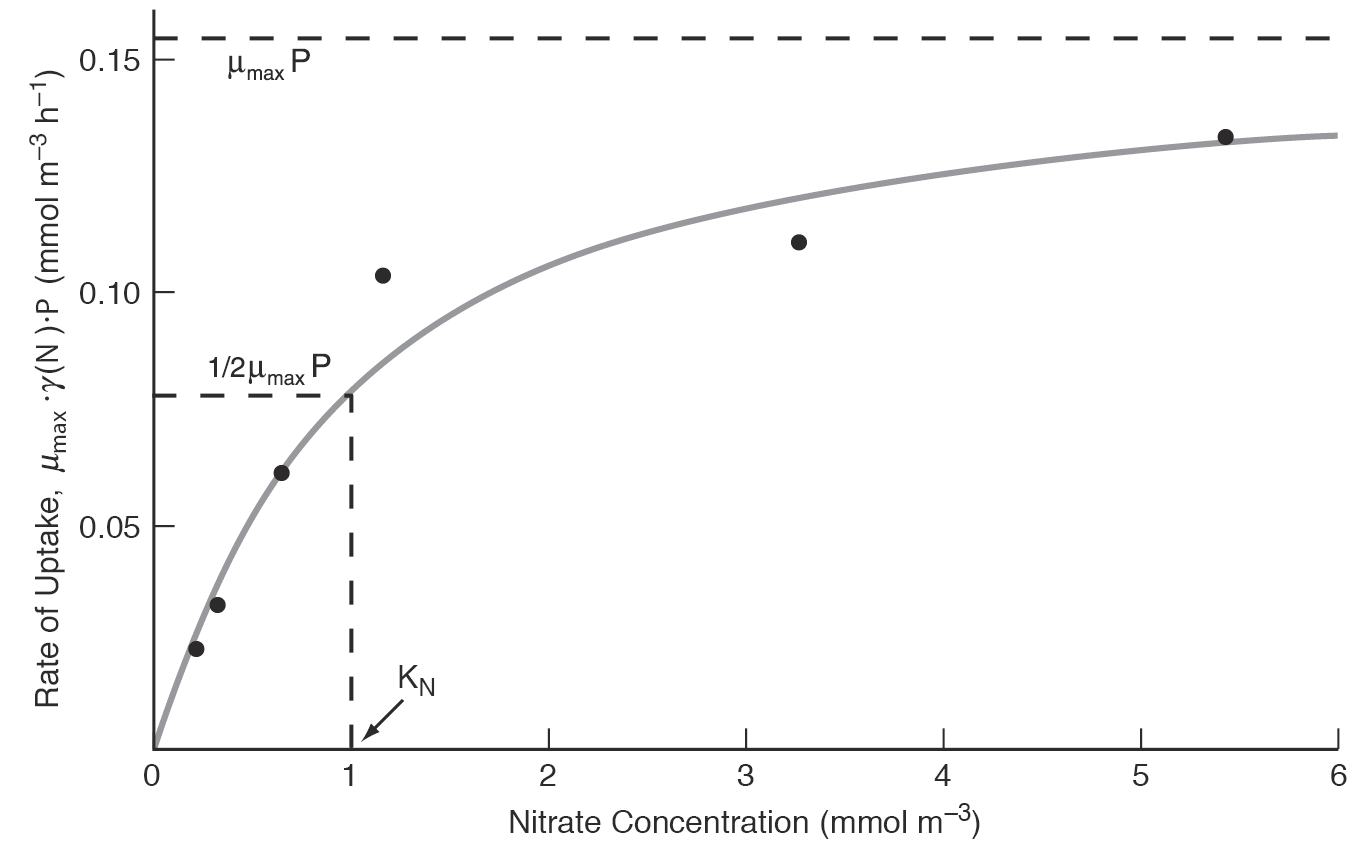
\includegraphics[width=5cm]{figures/MM}

{\footnotesize{}It's easier to compute the derivative if the Monod
function is rearranged in the following way
\[
\mu\left(N\right)=\mu_{max}\frac{N}{N+K_{N}}=\underbrace{\mu_{max}N}_{f_{1}}\underbrace{\left(N+K_{N}\right)^{-1}}_{f_{2}}
\]
to see the product of two functions.}{\footnotesize\par}

\column{8cm}
\begin{itemize}
\item {\footnotesize{}Computing the derivative of the growth function requires
some algebra 
\begin{align*}
\mu'\left(N\right) & =\mu_{max}\left(N+K_{N}\right)^{-1}-\mu_{max}N\left(N+K_{N}\right)^{-2}\\
 & =\frac{\mu_{max}}{N+K_{N}}\left(1-\frac{N}{N+K_{N}}\right)=\mu_{max}\frac{K_{N}}{\left(N+K_{N}\right)^{2}}
\end{align*}
}{\footnotesize\par}
\item {\footnotesize{}It is very useful to understand that the maximum increase
in uptake rate is obtained when the concentration is close to 0. The
slope of the function at $N=0$ is $\mu_{max}/K_{N}$ and it decreases
for each value of $N>0$ (you call it the gradient, but be careful
that this term has a precise meaning as we'll learn in SEA3004F).}{\footnotesize\par}
\end{itemize}
\end{columns}

\end{frame}


\subsection{Not just one driver}

\frame{\subsectionpage}
\begin{frame}{The functionality cascade}

\begin{itemize}
\item <1->Density in the ocean is a function of temperature, salinity and
pressure $\rho=f\left(T,S,P\right)$
\item <2->Temperature and salinity are functions of space and time $T=f\left(x,y,z,t\right)$
\item <3->Density is an indirect function of space and time $\rho=g\left(x,y,z,t\right)$
(as well as temperature and salinity)
\item <4->It is difficult to derive (pure) primitive equations, this is
why we need to use mathematical functions to express (parameterize)
relationships
\end{itemize}
\end{frame}

\begin{frame}{Functions of more than one variable}

\begin{definition}
A function of two or more variables is called \textbf{multivariate
(or multi-variables)}
\end{definition}

\begin{itemize}
\item Most of the oceanographic and atmospheric variables are multivariate
\item They are functions of space (the 3 independent variables $x,\,y,\,z$)
and time (\emph{these are variables, but not drivers!})
\item Most physical and biological processes are multivariate because they
\textbf{depend on more than one }\textbf{\emph{independent}}\textbf{
driver }\textbf{\scriptsize{}Q: do you remember the difference between
dependent and independent variables? Why the Cartesian axes are variables?}{\scriptsize\par}
\end{itemize}
\end{frame}

\begin{frame}{Interactive effects in biogeochemistry}

\begin{itemize}
\item {\footnotesize{}Phytoplankton growth is controlled by multiple interacting
drivers. Nutrients are abundant in the deeper ocean but light availability
does not allow to attain the maximum rate of photosynthesis. Micronutrients
may also play a role and temperature or ocean acidification can ultimately
affect physiological rates in certain species.}{\footnotesize\par}
\end{itemize}
\begin{example}
{\footnotesize{}In a warmer ocean, we may expect quicker physiological
metabolism and an increase in surface stratification. This will enhance
light availability because the cells are more likely to spend time
in the illuminated ocean layer, but it will reduce nutrient supply
from the deeper ocean because of the reduction in mixing rates. The
final effect can thus be either }\emph{\footnotesize{}aggravating}{\footnotesize{}
or }\emph{\footnotesize{}mitigating}{\footnotesize{} depending on
the relative change of each driver and their combined effect.}{\footnotesize\par}
\end{example}

\begin{itemize}
\item {\footnotesize{}These drivers have thus an }\textbf{\footnotesize{}interactive
effect}{\footnotesize{}, which is mostly described in terms of a }\textbf{\footnotesize{}multiplicative
effect}{\footnotesize{}. If each reaction norm is nonlinear, the resulting
combination can lead to surprising effects, which are hard to tackle
in laboratory experiments where we can manipulate a limited number
of drivers (}{\footnotesize{}\uline{\href{https://onlinelibrary.wiley.com/doi/full/10.1111/gcb.14102}{Boyd et al., 2018}}}{\footnotesize{})}{\footnotesize\par}
\end{itemize}
\end{frame}
%
\begin{frame}{Multiplicative effects due to combined resource limitation}
\begin{itemize}
\item <1->{\small{}We will consider a simplified case in which phytoplankton
nutrient uptake is controlled both by temperature and by nutrient
availability. The Lassiter function can be used to represent the temperature
reaction norm and the Michaelis-Menten equation the response to nutrient
\[
\mu\left(T,N\right)=\mu_{max}f(T)\,g(N)
\]
with $f(T)$ and $g(N)$ both non-dimensional functions}{\small\par}
\item <2->{\small{}The Lassiter equation is however complicated to manipulate,
and we can use another parameterization that is often used to represent
how physiological rates are affected by temperature. The $Q_{10}$
}{\small{}\uline{\href{https://en.wikipedia.org/wiki/Q10_(temperature_coefficient)}{coefficient}}}{\small{}
is the factor that multiplies the rate every 10$^{o}C$ change in
temperature
\[
\mu_{max}(T)=\mu_{10}Q_{10}^{\frac{T-10}{10}}
\]
}{\small\par}
\item <3->{\small{}If $Q_{10}\approx2$, as in many physiological processes,
the rate doubles every 10$^{o}C$. Bear in mind that this reaction
norm is different from the full convex function, since it assumes
monotonic increase with temperature.}{\small\par}
\end{itemize}
\end{frame}
%
\begin{frame}{Co-limitation: a simple parameterization}
\begin{columns}[t]
%

\column{8cm}
\begin{itemize}
\item {\small{}We thus construct the following parameterization representing
co-limitation
\[
\mu(T,N)=\mu_{10}Q_{10}^{\frac{T-10}{10}}\frac{N}{N+K_{N}}
\]
which is a function of 2 variables (a map, also called a landscape). }{\small\par}
\item {\small{}This is an illustrative example of the response of the uptake
rate to concurrent variations of temperature and nutrient }{\small\par}
\item {\small{}Designing real experiments to test responses is more complicated.
Read more at }{\small{}\uline{\href{https://meddle-scor149.org/}{https://meddle-scor149.org/}}}{\small\par}
\end{itemize}

\column{7cm}

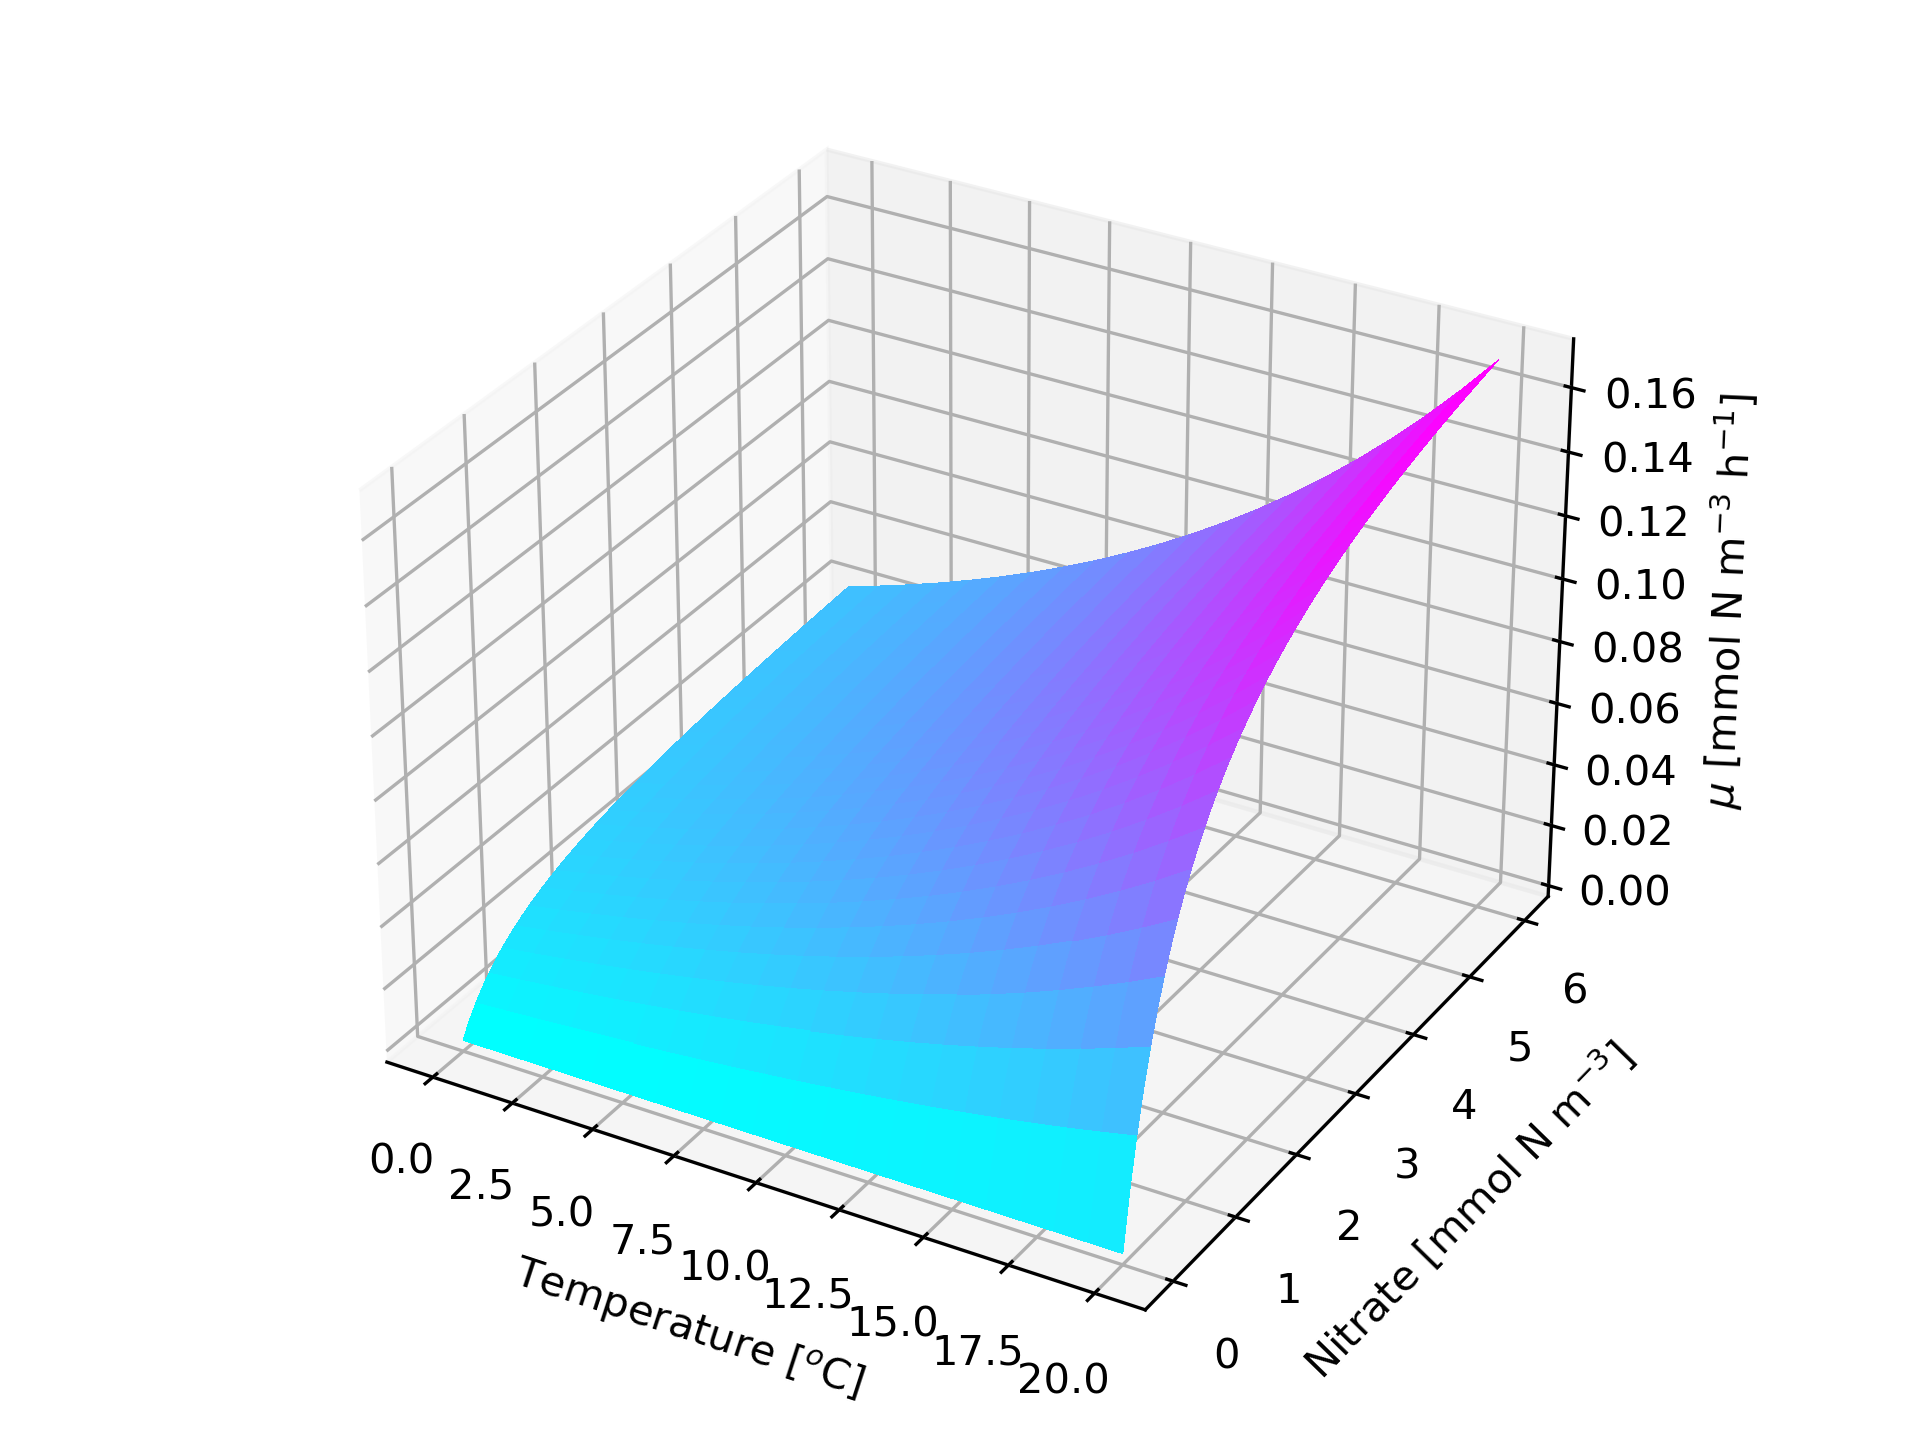
\includegraphics[width=8cm]{figures/multiplicative_effect}
\end{columns}

\end{frame}

\begin{frame}{The derivative of a multivariate function}

\begin{itemize}
\item {\footnotesize{}We can apply the concept of the derivative as the
change $df$ of $f\left(x\right)$ for infinitesimally small steps
$dx$ to a function of more than 1 variable}{\footnotesize\par}
\item {\footnotesize{}Function $g\left(x,y\right)$ depends on 2 independent
variables and is used to describe mathematically a map, like sea surface
temperature or nutrient concentration at regular spacing locations}{\footnotesize\par}
\item {\footnotesize{}To know the change along $x$ or $y$ we compute the
}\emph{\footnotesize{}partial derivative,}{\footnotesize{} indicated
with the symbol $\partial$ instead of the $d$
\[
\frac{\partial g}{\partial x},\frac{\partial g}{\partial y}\ \textrm{also}\ \partial_{x}g,\partial_{y}g\ \textrm{or even}\ g_{x},g_{y}
\]
}{\footnotesize\par}
\item {\footnotesize{}If the derivative is computed along space, it is called
the }\textbf{\footnotesize{}gradient}{\footnotesize{}. There may be
other independent variables over which the derivative is computed,
but you should be careful of using the term gradient only when referring
to spatial derivatives.}{\footnotesize\par}
\end{itemize}
\begin{definition}
\textbf{\footnotesize{}Partial derivatives}{\footnotesize{} are computed
by treating all independent variables, }\emph{\footnotesize{}other
than the variable with respect to which we are differentiating}{\footnotesize{},
as constants.}{\footnotesize\par}
\end{definition}

\end{frame}
%
\begin{frame}{Partial derivatives}
\begin{itemize}
\item A very good introduction to partial derivatives, and how they relate
to ordinary derivatives, is given by the \uline{\href{https://youtu.be/AXqhWeUEtQU}{Kahn Academy}}
\item A few exercises are available in the textbook \uline{\href{https://openstax.org/books/calculus-volume-3/pages/4-3-partial-derivatives}{Openstax Calculus (vol. 3)}}
(examples 4.15 and 4.18, also ex. 404 and 407)
\item Make sure that you spend some time to familiarize with the method
of computing derivatives, since multivariate (or multi-variable) functions
are common in ESS and will be used extensively in SEA3004
\end{itemize}
\end{frame}

\begin{frame}{Exploring the landscape}

\vspace{-2cm}
\begin{flalign*}
\mu(T,N)=\mu_{10}Q_{10}^{\frac{T-10}{10}}\frac{N}{N+K_{N}} &&
\end{flalign*}{\small{}You may need to watch }{\small{}\uline{\href{https://www.youtube.com/watch?v=Mci8Cuik_Gw}{this video}}}{\small{} }{\small\par}

{\small{}to review that $2^{x}=e^{x\ln2}$}{\small\par}

{\small{}and $\frac{d}{dx}2^{x}=\ln2\cdot2^{x}$}{\small\par}
\end{frame}
%
\begin{frame}{Nonlinear responses at different treatment levels}

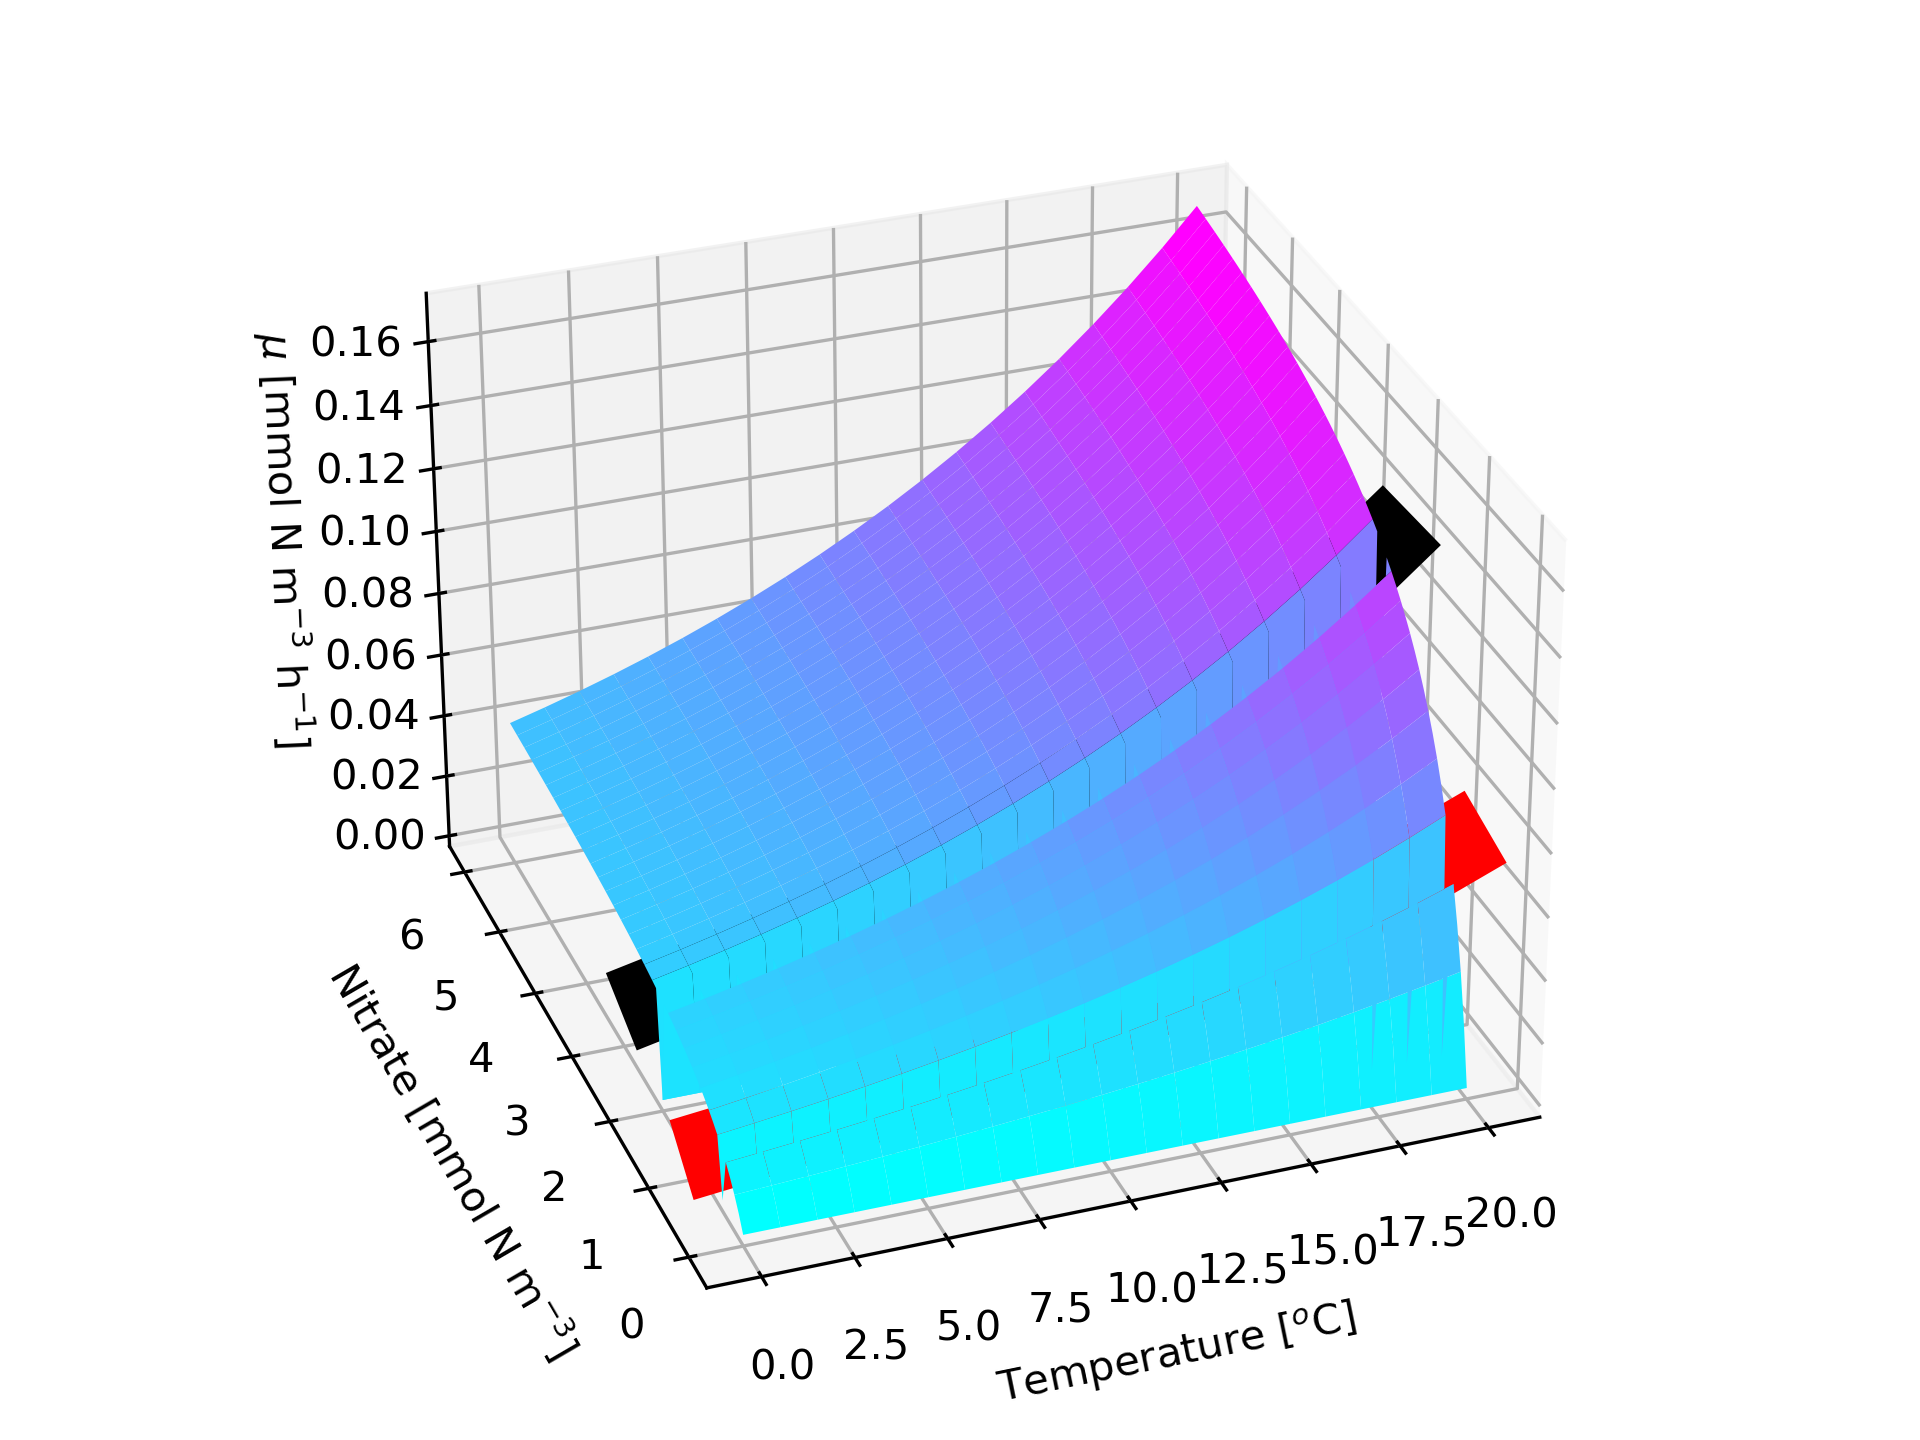
\includegraphics[width=8cm]{figures/multiplicative_effect_slice}
\end{frame}
%

\section{Introduction to differential equations}
\begin{frame}{Dynamical systems}

\begin{itemize}
\item <1->One branch of mathematics is dedicated to the analysis of \textbf{dynamical
systems}, and the ocean is certainly dynamical
\item <2->To describe dynamical systems we use differential equations.
They are equations in which the unknown is not a variable (or more),
but a function (or more)
\item <3->Two simple examples of ordinary differential equations are

\begin{itemize}
\item <3->growth dynamics
\item <3->light attenuation (or decay equation)
\end{itemize}
\end{itemize}
\end{frame}

\begin{frame}{Phytoplankton growth}

\begin{center}
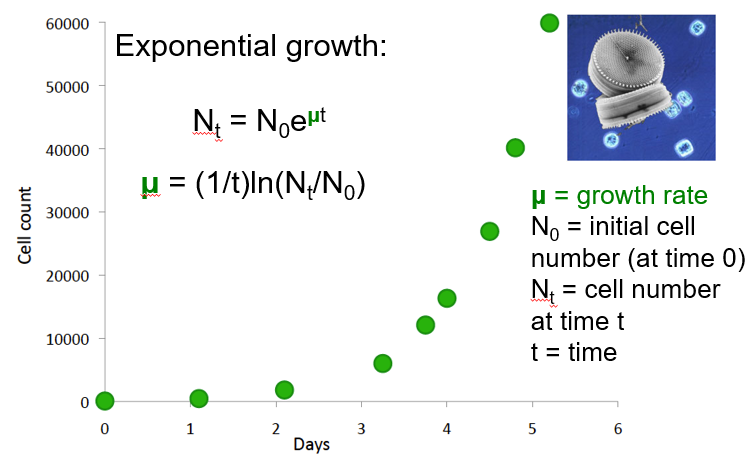
\includegraphics[scale=0.45]{figures/phytoplankton_growth}
\par\end{center}

{\tiny{}You've seen that cultured phytoplankton follow an exponential
growth, from which it is possible to estimate the growth rate. This
information can be used to infer how the cells would grow in the natural
environment. However, in a laboratory we can only control a few of
the environmental drivers.}{\tiny\par}
\end{frame}

\begin{frame}{Ordinary Differential Equations (ODE)}

\begin{definition}
ODEs are mathematical objects useful to describe changes in time or
in space because they are based on one single independent variable
\[
\frac{dC}{dt}=f\left(C,t,\mathsf{constants}\right);\ \frac{dC}{dx}=f\left(C,x,\mathsf{constants}\right)
\]
\end{definition}

\begin{itemize}
\item <1->A full introduction to ODEs is available at this online resource:
\uline{\href{https://openstax.org/books/calculus-volume-2/pages/4-introduction}{Openstax Calculus (volume 2)}}
(excluding Sec. 4.2)
\item <2->{\small{}In practice, we will encounter 2 types of ODEs:}

\begin{itemize}
\item <2->\textbf{\small{}0-dimensional (time)}{\small{}: this model describes
the time evolution of a variable (temperature, phytoplankton population,
etc.). }{\small\par}
\item <2->\textbf{\small{}1-dimensional (space)}{\small{}: light attenuation
is an example of 1-D spatial ODE. The solution is a spatial distribution
(in this case a profile).}{\small\par}
\end{itemize}
\end{itemize}
\end{frame}

\begin{frame}{Population growth}

\begin{itemize}
\item <1->In 1798, Thomas R. Malthus suggested that human population would
grow of a fixed proportion over a given amount of time in the absence
of external constraints
\item <2->This was the beginning of ``population ecology'' and it was
the first time that one of the basic principles of population dynamics
were enunciated
\item <3->Malthusian growth (or exponential growth) states that the time
rate of change of the population is proportional to the size of the
population itself
\item <4->This model describes the growth of microorganisms (bacteria,
phytoplankton) or virus in a \emph{continuous culture;} or any demographic
population \emph{in the unrealistic case of infinite resources}. It
is a typical example of a \textbf{0-dimensional Ordinary Differential
Equation} 
\end{itemize}
\end{frame}

\begin{frame}{Maltusian growth model}

\begin{itemize}
\item <1->The derivation of the Malthusian model is based on the concept
that growth is proportional to the population. The independent variable
is time and there is an increase of population with time that can
be written 
\[
\Delta N=\mu N\Delta t
\]
\item <2->We rewrite this principle in differential form by assuming that
$N$ is a continuous variable (if abundance, it's discrete). We obtain
what is called the \emph{dynamics for exponential growth} \emph{\vspace{-0.3cm}
\begin{flalign*}
\frac{dN}{dt}=\mu N
\end{flalign*}
}
\item <3->It can be solved analytically by separation of variables, integrating
the two sides and applying the initial condition $N(t=0)=N_{0}$\begin{flalign*}
\int\frac{1}{N}dN&=\mu\int dt\Rightarrow N=N_{0}e^{\mu t}&&
\end{flalign*}
\end{itemize}
\end{frame}

\begin{frame}{Population models}

\begin{columns}[t]


\column{6cm}
\begin{itemize}
\item {\small{}Maltusian growth can be further divided in a combination
of constant growth and loss terms acting on the population
\[
\frac{dN}{dt}=\left(r-d\right)N
\]
}{\small\par}
\item {\small{}This equation has one trivial solution for $N=0$. }{\small\par}
\item {\small{}What happens when $r=d$?}{\small\par}
\item {\small{}Up to 1870 growth in the US was Malthusian with $\mu=1.351\ y^{-1}$}{\tiny{}
}\linebreak{}
{\tiny{}(http://www-rohan.sdsu.edu/\textasciitilde jmahaffy/courses/f00/math536/dynamic/}\linebreak{}
{\tiny{}population/pop1\_model.html)}{\tiny\par}
\end{itemize}

\column{5.5cm}

\vspace{-1cm}
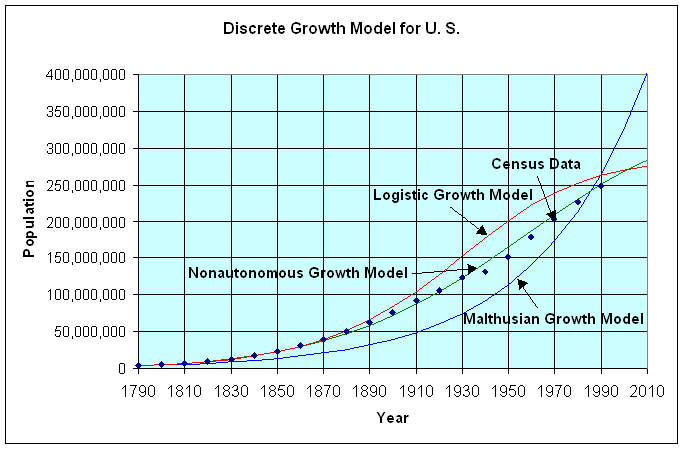
\includegraphics[width=5.2cm]{figures/usmodels}

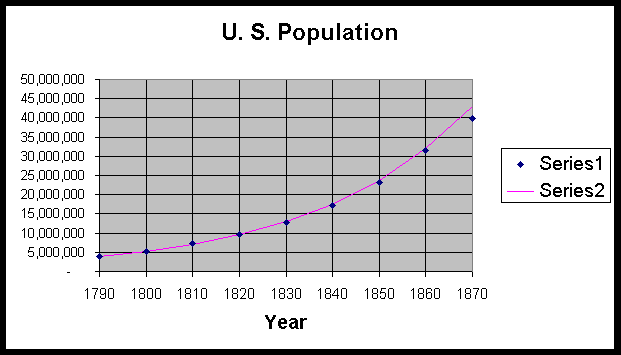
\includegraphics[viewport=10bp 10bp 500bp 340bp,clip,scale=0.25]{figures/uspop1870}
\end{columns}

\end{frame}

\begin{frame}{An equation for light attenuation}

\begin{itemize}
\item <1->It took 3 scientists to lay out the details of a rather simple
concept: the propagation of light through a medium is a linear function
of the incident light intensity
\item <2->Bouger first attempted to understand the \textquotedbl amount\textquotedbl{}
of light (energy) that was dissipated as light \textquotedbl descended\textquotedbl{}
into Earth's atmosphere, then Lambert developed the concept and Beer,
100 years later made it mathematically general (See more at: \href{http://www.ams.org/samplings/feature-column/fcarc-climate}{http://www.ams.org/samplings/feature-column/fcarc-climate}).
\item <3->The mathematical model of light attenuation in the case of a
constant medium (like glass) is a typical model of a physical process
based on a \textbf{1-dimensional ODE} 
\end{itemize}
\end{frame}

\begin{frame}{Light attenuation in ocean waters}

\begin{center}
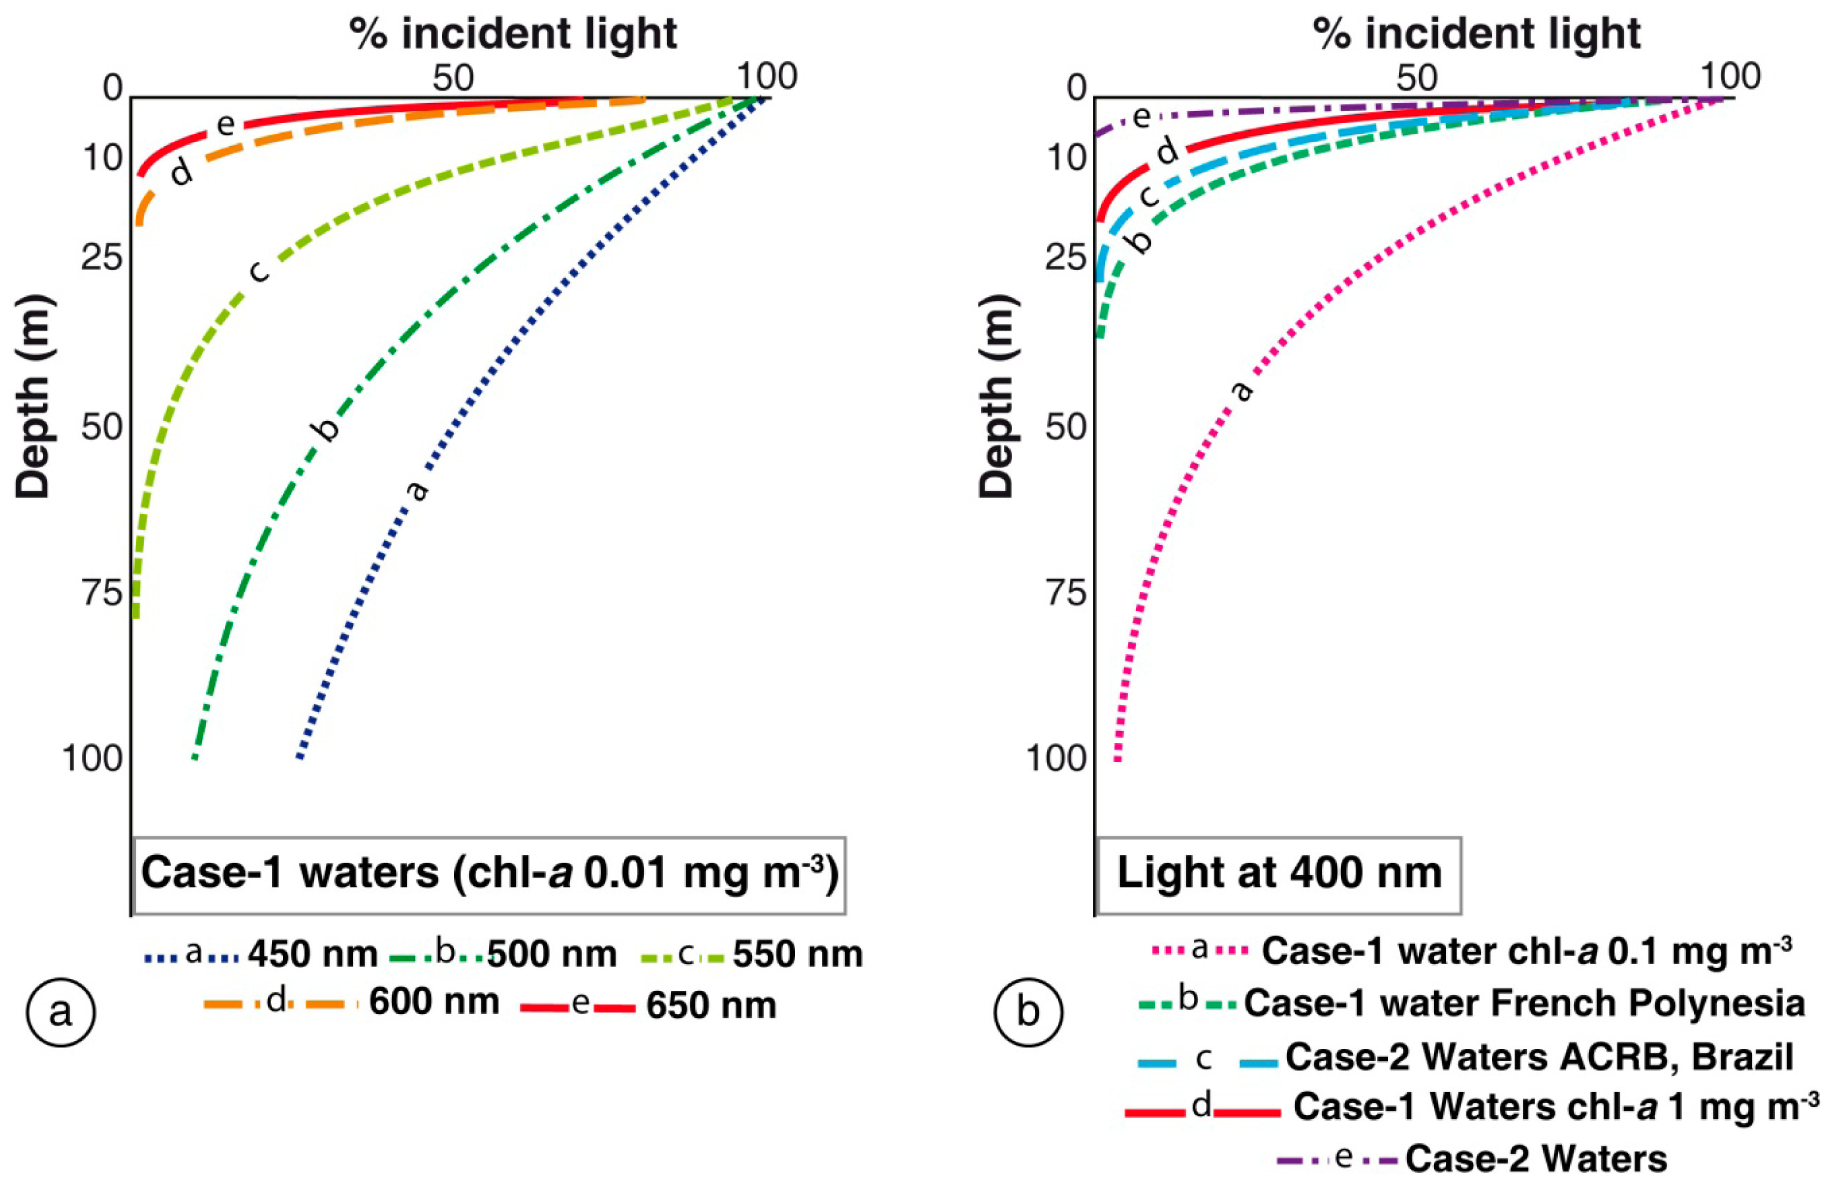
\includegraphics[scale=0.9]{figures/light_extinction}
\par\end{center}
\begin{itemize}
\item {\footnotesize{}Attenuation profiles for different wavelength and
types of waters (case 1, clear waters; case 2, coastal waters ; Zoffoli
et al., 2014, doi:10.3390/s140916881)}{\footnotesize\par}
\end{itemize}
\end{frame}

\begin{frame}{Lambert-Beer equation}

\begin{columns}[t]


\column{8cm}
\begin{itemize}
\item {\footnotesize{}Light is attenuated of a certain fraction in its pathway
through the medium, which is characterized by the constant attenuation
coefficient $\varepsilon$ (units?)
\[
I_{1}=I_{0}-\varepsilon I_{0}\ell\Rightarrow\Delta I=-\varepsilon I\Delta x
\]
}{\footnotesize\par}
\end{itemize}

\column{4cm}

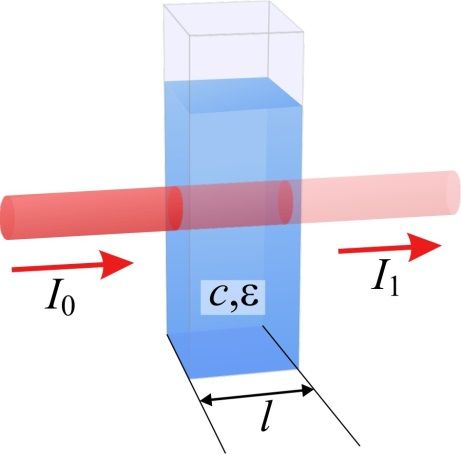
\includegraphics[scale=0.6]{figures/lambert-beer}
\end{columns}

\begin{itemize}
\item {\footnotesize{}By putting it in differential form, one obtains the
Lambert-Beer equation
\[
\frac{dI}{dx}=-\varepsilon I
\]
which can be solved analytically by separating the variables, integrating
the two sides and applying the boundary condition $I(x=0)=I_{0}$
\[
\int\frac{1}{I}dI=-\varepsilon\int dx\Rightarrow I=I_{0}e^{-\varepsilon x}
\]
}{\footnotesize\par}
\end{itemize}
\end{frame}

\begin{frame}{ODE features for future reference (see Openstax Calculus vol. 2)}

\begin{itemize}
\item {\scriptsize{}the }\textbf{\scriptsize{}order}{\scriptsize{} is the
value of the highest-order derivative
\[
\frac{dC}{dt}=\lambda C^{3}-C^{2}+a_{0}\ \left(\mathsf{1st}\right);\ \frac{d^{2}C}{dx^{2}}=\mu\frac{dC}{dx}-C\ \left(\mathsf{2nd}\right)
\]
}{\scriptsize\par}
\item {\scriptsize{}a }\textbf{\scriptsize{}homogeneous}{\scriptsize{} (or
autonomous) ODE has only terms containing the dependent variable or
its derivative $\frac{dC}{dt}=-\lambda C$}{\scriptsize\par}
\item {\scriptsize{}a }\textbf{\scriptsize{}non-homogeneous}{\scriptsize{}
(or non-autonomous) ODE contains additional terms, such as constants
or the independent variable itself
\[
a_{2}\frac{d^{2}C}{dx^{2}}+a_{1}\frac{dC}{dx}-a_{0}C=x^{2}
\]
}{\scriptsize\par}
\item {\scriptsize{}a }\textbf{\scriptsize{}linear}{\scriptsize{} ODE only
contains linear terms, like the population growth. If the variable
has an exponent, then the ODE becomes }\textbf{\scriptsize{}nonlinear}{\scriptsize{}.
\[
\frac{dN}{dt}=\mu N-dN^{2}
\]
}{\scriptsize\par}
\item \textbf{\scriptsize{}initial value problems}{\scriptsize{} have a
starting point $C(t=t_{0})=C_{0}$ and are }\emph{\scriptsize{}integrated}{\scriptsize{}
forward in time to obtain $C(t)$ (for all) $\forall t>t_{0}$}{\scriptsize\par}
\item \textbf{\scriptsize{}boundary value problems}{\scriptsize{} seek the
solution $C(x)$ over a certain domain given specific values at the
beginning and end of the domain $\left(C(x=x_{b})=C_{0};C(x=x_{e})=C_{1}\right)$
or even within the domain itself}{\scriptsize\par}
\end{itemize}
\end{frame}


\section{Examples of mathematical models}

\frame{\subsectionpage}
\begin{frame}{Limits to growth}
\begin{itemize}
\item <1->Scientists quickly realized that Malthusian growth is not an
adequate model to describe the time evolution of populations. A population
cannot grow indefinitely, and various constraints may emerge. The
availability of environmental resources is a major limiting factor,
which can be expressed in terms of nutritional resources or space
resources
\item <2->Not only bottom-up growth, but also top-down control can play
a role (ecological interactions)
\item <3->The physical environment can exert a considerable pressure at
various scales, and organisms/communities have built their specific
ecological strategies to survive and to strive
\end{itemize}
\end{frame}

\begin{frame}{Simple mathematical models}

\begin{itemize}
\item \textbf{The logistic model and the carrying capacity}
\item The Lotka-Volterra model of prey-predator interactions
\item The Sverdrup model of phytoplankton bloom
\end{itemize}
\end{frame}
%
\begin{frame}{Other types of growth: the logistic model}
\begin{itemize}
\item <1->The logistic model assumes that a population would asymptotically
tend towards a stable value, that is the maximum ``abundance'' that
a particular environment can sustain indefinitely
\item <2->This number is called the \textbf{carrying capacity} and the
logistic model of a continuous population $N(t)$ is expressed as
\begin{flalign*}
\frac{dN}{dt}=rN\left(1-\frac{N}{K}\right) &&
\end{flalign*}
\item <3->A full introduction on the need to move away from unconstrained
growth and the concept of limited growth is given in this very good
lecture from the \uline{\href{https://www.khanacademy.org/math/ap-calculus-bc/bc-differential-equations-new/bc-7-9/v/modeling-population-with-differential-equations}{Kahn Academy}}
(especially the first two videos)
\end{itemize}
\end{frame}
%
\begin{frame}{The solution of the logistic ODE}
\begin{columns}[t]

\column{8cm}

The analytical solution of this differential equation is the logistic
curve
\[
N\left(t\right)=\frac{N_{0}Ke^{rt}}{K+N_{0}\left(e^{rt}-1\right)}=\frac{N_{0}K}{N_{0}+\left(K-N_{0}\right)e^{-rt}}
\]
where $N_{0}$ is the initial population value (the initial condition).
This solution, which is often called the sigmoid curve, is shown for
various values of $N_{0}$. 

\column{6cm}

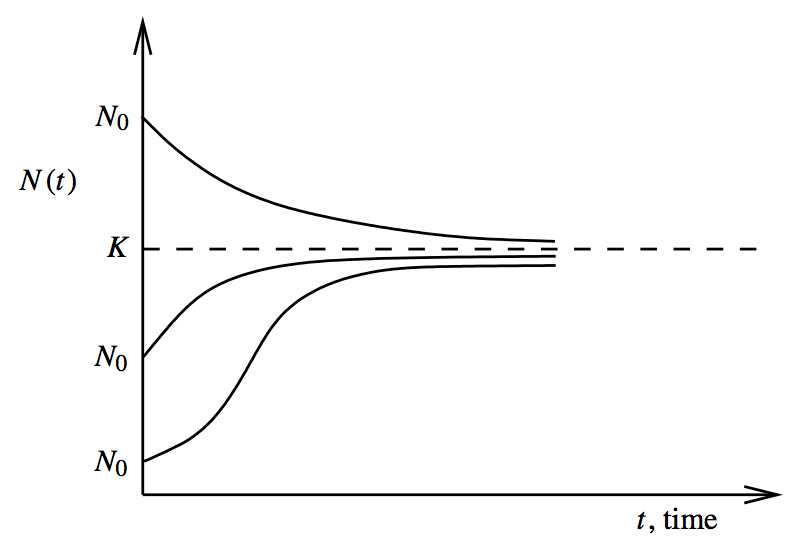
\includegraphics[width=5cm]{figures/logistics}

Note the qualitative difference for the two cases $N_{0}<K/2$ and
$K>N_{0}>K/2$.
\end{columns}

\end{frame}

\begin{frame}{Analysis of the logistic model}
\begin{columns}[t]
%

\column{5cm}
\begin{enumerate}
\item {\scriptsize{}Indicate the order of this differential equation}{\scriptsize\par}
\item {\scriptsize{}If the equation is expressed in SI concentration units
with biomass in kg m$^{-3}$, what are the units of $r$ and $K$?}{\scriptsize\par}
\item {\scriptsize{}Identify the linear and non linear terms and briefly
explain which ecological processes they may represent}{\scriptsize\par}
\item {\scriptsize{}From the figure, what is the meaning of $K$ and what
would happen if $N_{0}=K$?}{\scriptsize\par}
\item {\scriptsize{}What happens to the equation if the carrying capacity
is very large $\left(K\rightarrow+\infty\right)$?}{\scriptsize\par}
\end{enumerate}

\column{9cm}

\begin{flalign*}
\frac{dN}{dt}=rN\left(1-\frac{N}{K}\right) &&
\end{flalign*}
\end{columns}

\end{frame}

\begin{frame}{Simple mathematical models}

\begin{itemize}
\item The logistic model and the carrying capacity
\item \textbf{The Lotka-Volterra model of prey-predator interactions}
\item The Sverdrup model of phytoplankton bloom
\end{itemize}
\end{frame}
%
\begin{frame}{Modelling ecological interactions}
\begin{itemize}
\item The use of mathematical models to describe biological interactions
has a long history, and it can be traced back to the analysis of the
oscillations occurring between preys and their predators.
\item This video from the \uline{\href{https://www.khanacademy.org/science/high-school-biology/hs-ecology/hs-ecological-relationships/v/predator-prey-cycle}{Kahn Academy}}
illustrates the expected dynamics when a population of predators 
\item This dynamics was originally studied at the beginning of 1900 by Lotka
and Volterra independently. It represents the most classical example
of a system of ODEs, in which we have one dynamics for each component
of the system
\end{itemize}
\end{frame}
%
\begin{frame}{The Lotka-Volterra model}
\begin{itemize}
\item <1->The model describes the interaction between two populations.
The prey $X_{1}$ grows following the Malthusian equation and is consumed
by the predator $X_{2}$ . The latter dies according to a constant
decay term. The model has 2 equations, one for each state variable
and 3 parameters
\begin{align*}
\frac{dX_{1}}{dt} & =X_{1}\left(p_{1}-p_{2}X_{2}\right)\\
\frac{dX_{2}}{dt} & =X_{2}\left(p_{2}X_{1}-p_{3}\right)
\end{align*}
\item <2->The system does not conserve mass. There is an infinite source
of energy that sustains the prey population and there is an infinite
sink for the predator mortality
\end{itemize}
\end{frame}

\begin{frame}{The model assumptions}
\begin{itemize}
\item \textbf{Please note that, although it has been applied in several
cases, it should be used as an illustrative model since it has major
assumptions} 
\end{itemize}
\begin{enumerate}
\item The species coexist in the same environment
\item The prey population is not resource limited 
\item The food supply of the predator population depends entirely on the
prey populations
\item The predator mortality is proportional to the population size
\item The environment does not change as well as the type of preys and predators.
\end{enumerate}
\end{frame}

\begin{frame}{A numerical solution for an ocean case}

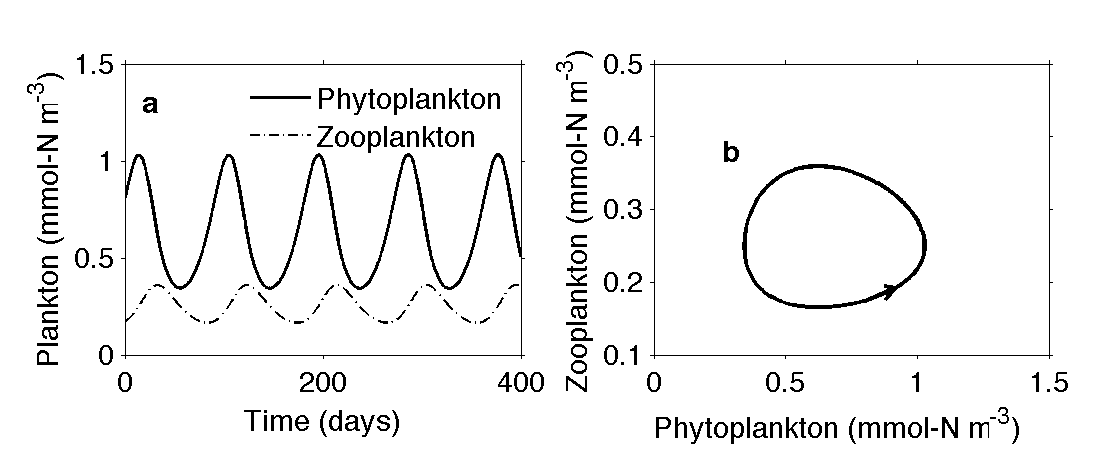
\includegraphics[scale=0.5]{figures/ftut_LVpzts1}

The LV model is nowadays used mostly for educational purposes, because
it allows a rigorous analysis to illustrate the major aspects of mathematical
biology and it is a tractable example of a numerical solution for
an ODE system. Moreover, it does contain elements that are common
to any marine biogeochemistry model.
\end{frame}

\begin{frame}{Simple mathematical models}

\begin{itemize}
\item The logistic model and the carrying capacity
\item The Lotka-Volterra model of prey-predator interactions
\item \textbf{The Sverdrup model of phytoplankton bloom}
\end{itemize}
\end{frame}
%
\begin{frame}{The Sverdrup model for phytoplankton bloom}
\begin{columns}[t]
%

\column{8cm}
\begin{itemize}
\item {\scriptsize{}In an influential paper published in 1953, Sverdrup
proposed that phytoplankton blooms occur in the ocean when there is
a vertical scale (where light availability decay exponentially) in
which biomass growth exceeds losses }{\scriptsize\par}
\item {\scriptsize{}He argued that if vertical mixing allows the cells to
stay in the illuminated layer for enough time to overcome their loss
rate, a bloom would develop}{\scriptsize\par}
\item {\scriptsize{}The power of this simple model is not in its predictive
capability. There are so many different drivers that can influence
phytoplankton blooms and they cannot be all included in a simple model.
}\textbf{\scriptsize{}This model represents the first attempt at combining
interdisciplinary concepts, such as turbulence and biological growth}{\scriptsize\par}
\item {\scriptsize{}There is an excellent }{\scriptsize{}\uline{\href{https://tos.org/oceanography/article/sixty-years-of-sverdrup-a-retrospective-of-progress-in-the-study-of-phytopl}{review paper}}}{\scriptsize{}
written by graduate students that illustrates the role played by the
Sverdrup model in oceanography. }{\scriptsize\par}
\end{itemize}

\column{6cm}

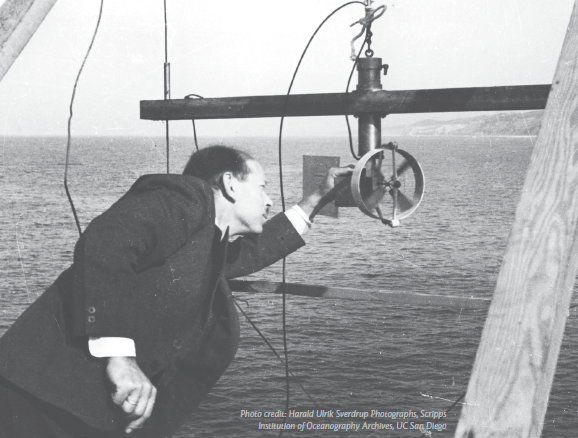
\includegraphics[width=5cm]{figures/sverdrup}
\end{columns}

\end{frame}

\begin{frame}{The critical depth hypothesis }
\begin{columns}[t]

\column{8 cm}

\textbf{Sverdrup's assumptions}
\begin{itemize}
\item A thoroughly mixed surface layer
\item Phytoplankton are evenly distributed in the mixed layer
\item Production in the mixed layer is only limited by light (no effects
of nutrients, temperature, grazing, etc.)
\item The attenuation coefficient for light remains constant throughout
the water column
\end{itemize}

\column{6 cm}

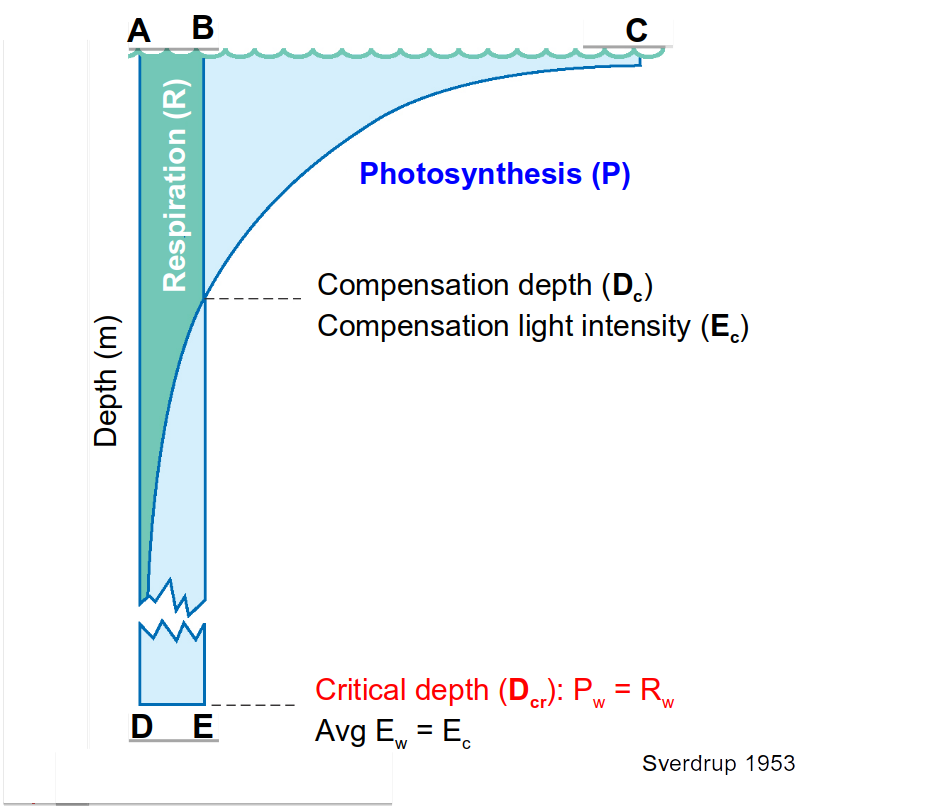
\includegraphics[width=7cm]{figures/Sverdrup_Fawcett}
\end{columns}

\end{frame}
%
\begin{frame}{A simplified version of the Sverdrup equations}
\begin{itemize}
\item <1->Phytoplankton biomass is represented by the 2-D function $P(t,z)$
\item <2->The growth rate is not constant because it depends on light availability.
Light decays exponentially with depth according to an attenuation
coefficient (note that the vertical coordinate is oriented upward,
$z$is altitude, which is negative below the water)
\[
r\left(t,z\right)=r_{max}e^{kz};\,d(t,z)=d_{0}
\]
\item <3->Being a multivariate function, we should use partial differential
equations and not ODE to describe the dynamics
\[
\frac{\partial P\left(t,z\right)}{\partial t}=\left[r\left(z\right)-d_{0}\right]P\left(t,z\right)
\]
\end{itemize}
\end{frame}
%
\begin{frame}{Interactions between physical and biological scales: critical depth}
\begin{columns}[t]

\column{8 cm}
\begin{itemize}
\item <1->{\footnotesize{}To make the problem treatable, we assume that
vertical mixing is much faster than biological growth in the water
column}{\footnotesize\par}
\item <2->{\footnotesize{}$P\left(t,z\right)$ is thus vertically homogeneous
and the same concentration of cells can be found at any depth in the
layer. }{\footnotesize\par}
\item <3->{\small{}Our state variable will be replaced by the average concentration
over depth $H$: $\hat{P}\left(t\right)=\frac{1}{H}\int_{-H}^{0}P(t,z)dz$
\begin{align*}
\frac{d\hat{P}}{dt} & =\frac{\hat{P}}{H}\int_{-H}^{0}\left(r_{max}e^{kz}-d_{0}\right)dz\\
 & =\frac{\hat{P}}{H}\left[r_{max}\int_{-H}^{0}e^{kz}dz-\int_{-H}^{0}d_{0}dz\right]
\end{align*}
}{\small\par}
\end{itemize}

\column{7 cm}

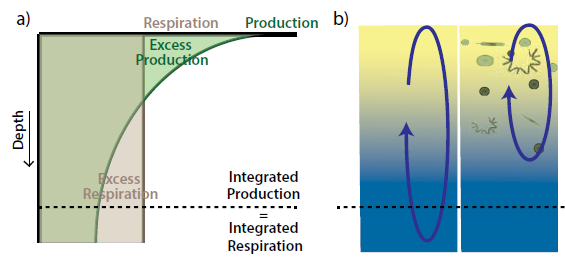
\includegraphics[width=6cm]{figures/sverdrup_fennel}
\begin{itemize}
\item <4->{\small{}We are now back to an ODE. The vertical integral on
the RHS is positive (i.e. growth) only above the depth where integrated
production is equal to integrated respiration. If the MLD is deeper
than the critical depth losses will dominate.}{\small\par}
\end{itemize}
\end{columns}

\end{frame}


\end{document}
